%****************************************************************
% Chapter X
%****************************************************************
\label{chapter-implementation}
\chapter{Implementation}

In this chapter, details of the major implementation are revealed. First, briefly introducing Google VR SDK setup and drawing with OpenGL ES. Then an explanation of the web server design. After that, the creation of 3D virtual scene is highlighted. Finally, the implementation for device movement and object intersection detection are  clarified.

%****************************************************************
\section{Google VR SDK}

The Google VR SDK repository is free and accessible from\href{https://github.com/googlevr/gvr-android-sdk}{\emph{https://github.com/googlevr/gvr-android-sdk}}, where we can get access to any necessary libraries and examples. The SDK libraries locate in the libraries directory of the repository as \emph{.aar} files \cite{google.aar-format.2016}. This project has two dependencies on \code{base} and \code{common} Google VR SDK modules.

%****************************************************************
\section{OpenGL ES}

OpenGL assumes a square coordinate system, by default, happily draws those coordinates onto the screen. However screens can vary in size and shape, that is to say, most screens are typically non-square screen. The illustration below \ref{fig:opengl-coordinates} shows the assumed uniform coordinate system of an OpenGL frame on the left, and how these coordinates map to an exemplary non-square device screen in landscape orientation on the right.

\begin{figure}[H]
\caption[OpenGL coordinate system mapping]{Default OpenGL coordinate system (left) mapped to a typical Android device screen (right) \cite{google.opengles.2016}}
\label{fig:opengl-coordinates}
\centering
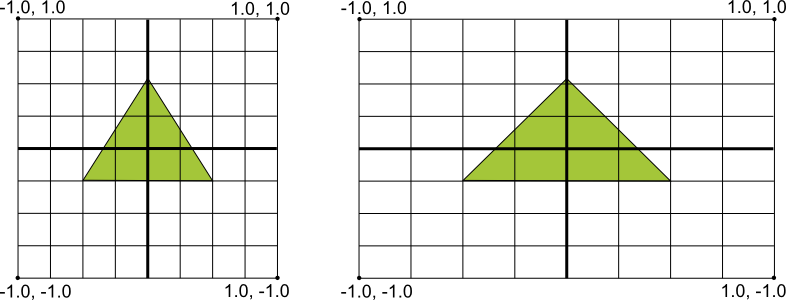
\includegraphics[width=\textwidth, keepaspectratio]{Figures/opengl-coordinates.png}
\decoRule
\end{figure}

Therefore, OpenGL projection modes and camera views have to be applied to the OpenGL rendering pipeline for coordinates transformation, so the graphic objects have the expected proportions on any display. The projection matrix will recalculate the coordinates of graphics objects, and the camera view matrix will create a transformation that renders objects from a specific eye position.

The implementation is divided into two phases. First, working out the model matrix, view matrix, and perspective matrix in CPU (Android programming in this case). Secondly pass them to GPU for the rest of calculation (OpenGL Shading Language Programming, i.e. GLSL or GLslang), such as explicit projection matrix, coordinates transformation, lighting, or more particular calculation (see \ref{section:ray}). The GLSL shaders themselves are a set of strings that passed to the hardware driver for compiling within an application using the OpenGL API's entry points \cite{wiki.glsl.2016}. By sharing the workload on CPU and GPU turns out significantly improved the performance, see Chapter Performance \ref{section:placemarks-update}.

\begin{table}[H]
\caption{OpenGL compute}
\label{tab:opengl-compute}
\centering
\begin{tabular}{l l l l}
\toprule
\tabhead{What} & \tabhead{How} & \tabhead{Where}\\
\midrule
Model Matrix & translationMx * scaleM * rotationM * identityM(1) & CPU\\
Camera Matrix & Matrix.setLookAtM(positionV, lookAtV, upV) & CPU\\
View Matrix & eye.getEyeView() * cameraM & CPU\\
Perspective Matrix & eye.getPerspective(zNear, zFar) & CPU\\
Projection Matrix & perspectiveM * viewM * modelM & GPU\\
Vertex' & projectionM * vertex & GPU\\
\bottomrule
\end{tabular}
\end{table}

%****************************************************************
\section{Web Server}

See the example below, a simple file server on port \code{8080} to serve a directory on disk "\emph{/tmp}" under an alternate URL path "\emph{/files/}", using \code{StripPrefix} to modify the request URL's path before the \code{FileServer} sees it.

\[
\begin{array}{lr}
\scriptsize{\code{http.Handle("/files/", http.StripPrefix("/files", http.FileServer(http.Dir("./tmp"))))}}\\
\scriptsize{\code{http.ListenAndServe(":8080"), nil)}}\\
\end{array}
\]

For RESTful APIs setup, I introduce a free framework Go-Json-Rest \cite{antoine.go-json-rest.2016}, it is a thin layer designed by KISS principle (Keep it simple, stupid) and on top of native net/http package that helps building RESTful JSON APIs even easier.

%****************************************************************
\subsection{Assets}

The file server processes the requests and delivers the result (the particular file) in a standard web format back to the client. Table \ref{tab:assets-structure} indicates the folder structure served by the server.

\begin{table}[H]
\caption{Assets structure}
\label{tab:assets-structure}
\centering
\begin{tabular}{l l l}
\toprule
\tabhead{Path} & \tabhead{Usage}\\
\midrule
\textbackslash assets & Root\\
\textbackslash assets\textbackslash static.zip & The compressed Patch (see \ref{section:patch}) \\
\textbackslash assets\textbackslash static\textbackslash kml & KML storage (see \ref{section:kml})\\
\textbackslash assets\textbackslash static\textbackslash layer & KML storage (see \ref{section:scene})\\
\textbackslash assets\textbackslash static\textbackslash model & Extra model storage (see \ref{section:obj-model})\\
\textbackslash assets\textbackslash static\textbackslash resource & Resource (eg. images) storage\\
\bottomrule
\end{tabular}
\end{table}

%****************************************************************
\subsection{Patch}
\label{section:patch}

A Path is for the server to guarantee the latest data (if any) will be pushed to each client (Android smartphone). It server as a compressed ZIP file, and it contains one or more files that require client to update. Patch validation is happening whenever the app starts. First, the client sent requests for the patch file "\emph{http://xxx.xxx.xxx.xxx:8080/assets/static.zip}" from the file server. Before actual download the file, take the \code{lastModifiedTime} data of remote Patch from HTTP response headers, and compare it with the other \code{lastModifiedTime} data of local's Patch file. Only when the local's Patch is out of date, the client continues to download the remote Patch file and replacing any existing local files. For a special scenario when the app was just installed in the first time launch, also the network is disconnected. A built-in default Patch that included in the APK (Android app binary) will be uncompressed to avoid no available data. Diagram \ref{fig:patch-check} shows the simplified process.

\begin{figure}[H]
\caption{Patch check}
\label{fig:patch-check}
\centering
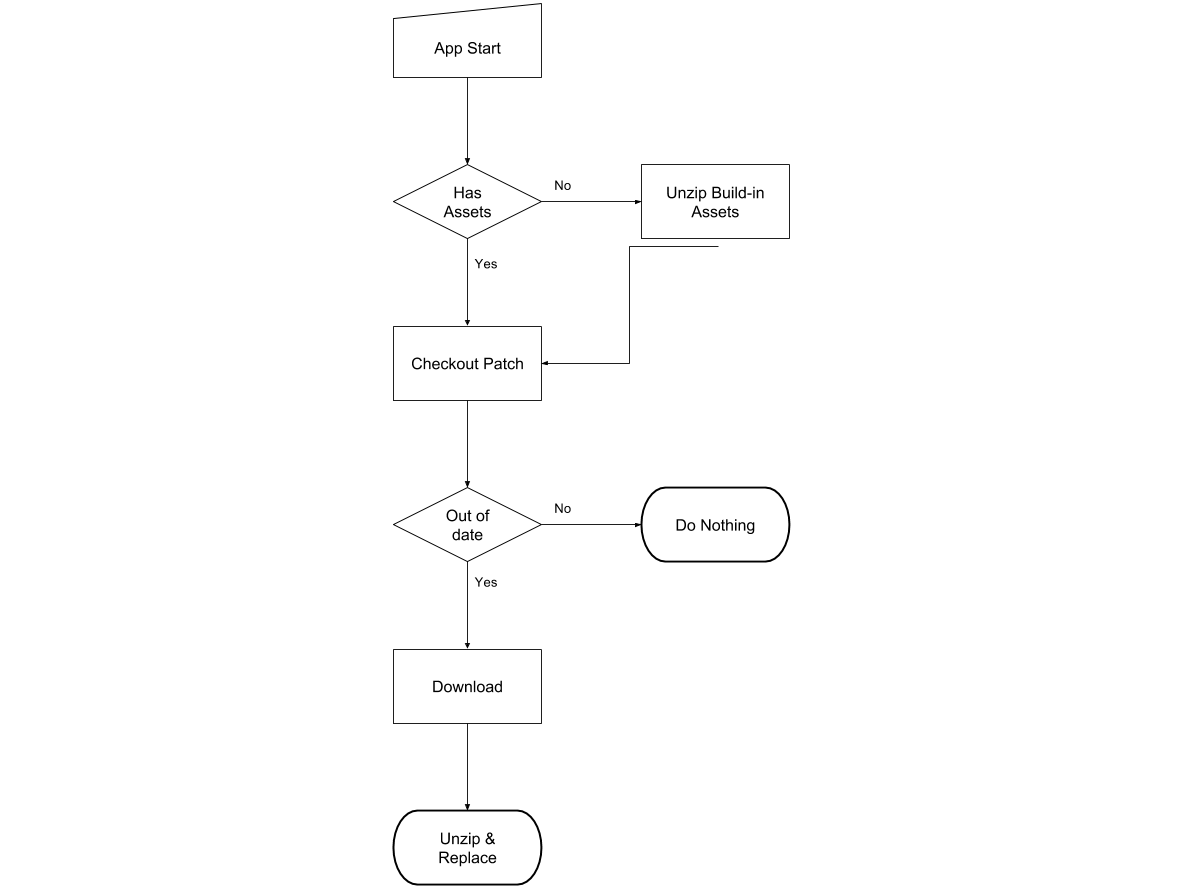
\includegraphics[width=\textwidth, keepaspectratio]{Figures/patch-check.png}
\decoRule
\end{figure}

%****************************************************************
\section{Scene}
\label{section:scene}

The Keyhole Markup Language (KML) is contributed to the application as the geographic visualization markup language. KML files from folder "\emph{/assets/static/layer} are visible to the user, and each KML file represents an individual 3D scene which contains any necessary geographic data related to the topic.

As you can see from Table \ref{tab:assets-structure}, there are two assets folders contains KML files - "\emph{/assets/static/layer}" and "\emph{/assets/static/kml}". These files are literally the same, but existing in different concepts for achieving the purpose of categorizing. By making use of \code{Networklink} facility, an individual KML file can contains one or more other KML files by given URLs. Therefore, folder "\emph{/assets/static/layer}" intends to be the scene topic (KML file) storage that visible and selectable to the user, and any inside topic could include one or more topics that exist in folder "\emph{/assets/static/kml}".

It has many advantages to dividing the space with certain patterns during the space creation. Such as, runtime graphical analysis and optimization, intersection and collision detection.

%****************************************************************
\subsection{Geographic Visualization Markup Language}
\label{section:kml}

There are only some of KML features from KML schema \ref{fig:kml-schema} are be used in this application. They are \code{Container}, \code{Style}, \code{Placemark}, and \code{NetworkLink}. The KML parser I am using is not coded from scratch, and it is based on the open-source library \code{android-maps-utils} \cite{google.code-kml.2016} but with certain modification and extension: getting rid of \code{GoogleMap} dependency; extending \code{NetworkLink} facility support that was one of the unsupported features in the library.

\begin{figure}[H]
\caption{kML parser simple}
\label{fig:kml-parser-simple}
\centering
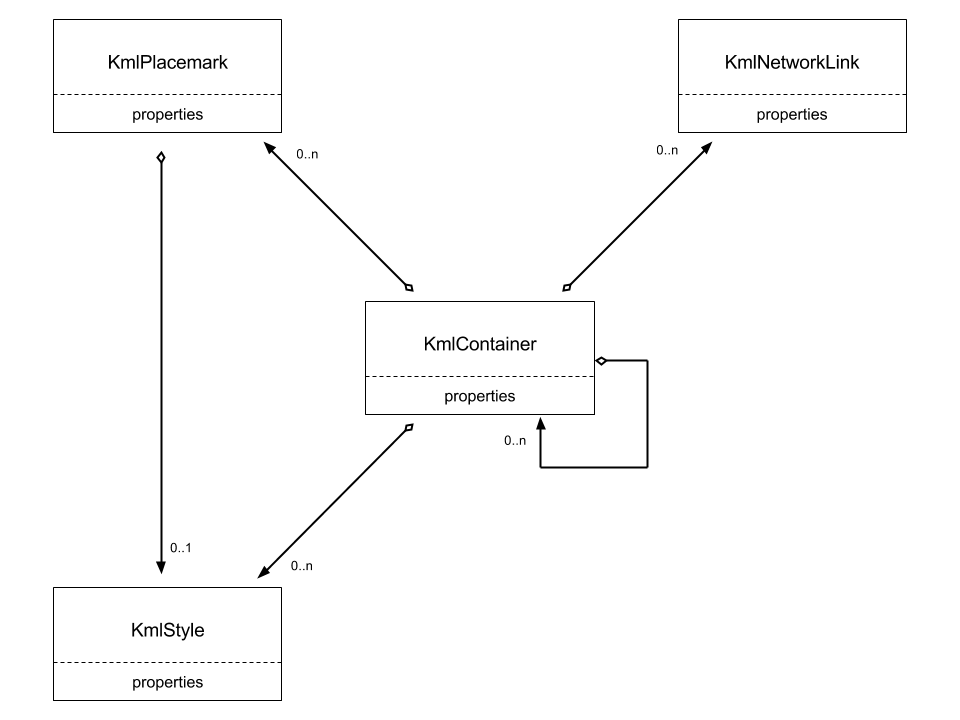
\includegraphics[width=\textwidth, keepaspectratio]{Figures/kml-parser-simple.png}
\decoRule
\end{figure}

%****************************************************************
\subsection{Space Partition} 
\label{section:space-partition}

Space partition often used for optimizing collision detection algorithms among polygonal models. These algorithms are often expensive operations and can significantly slow FPS down. Although there is no collision detection in this application yet, there is an intersection detection between the ray tracing (see \ref{section:ray}) and other objects. Space partition is contributed to reducing the ray-object intersection test load by skipping invalid objects that locate far away from current ray tracing area. It avoids doing an $n^2$ times intersection detection on all objects.

A axis-aligned Octree is implemented for the space partition \ref{fig:octree-split}. It has a predefined constant positive integer to decide whether or not a new partitioning should happen. This number is important for the purpose of reducing intersection detections, and it indicates a minimum number of objects allowed exist in the same cell. In view of the object complexity (sphere) and the cell complexity (box), the number $5$ was adopted (see \ref{chapter-performance} for more details). 

\begin{description}
	\setlength{\parskip}{0pt}
	\item[$\bullet$ Object Complexity] \code{Plackmarker} is doing ray-sphere detection (see \ref{section:ray-sphere})
	\item[$\bullet$ Cell Complexity] Cell is doing ray-box detection (see \ref{section:ray-box})
\end{description}

If the number is positive infinity - whole space seen as a cell and no further space partition is required, this is not reduce anything but also increase to $n + 1$ times of detections ($n$ times for ray-object, $1$ times for ray-cell). If the number is $1$ - each cell only contains one object, this also not reduces the number of detection times, but increase to at least $2\,n$ times. Since the ray-box detection action is much cheaper then ray-sphere's, an appropriate value can eventually reduce the overall intersection detections.

\begin{figure}[H]
\caption{Octree division}
\label{fig:octree-division}
\centering
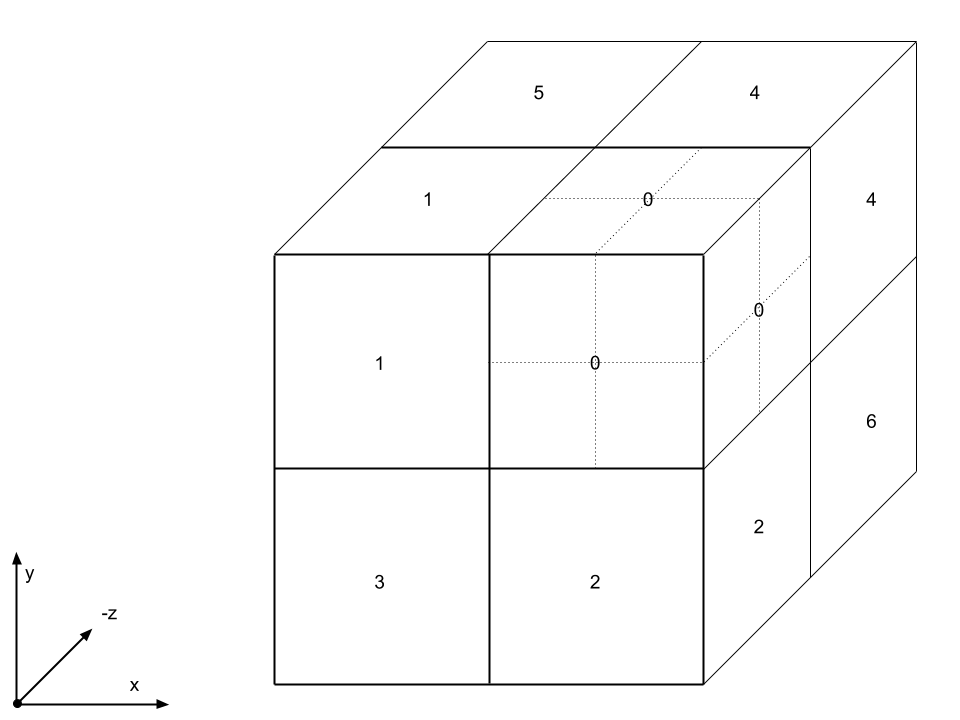
\includegraphics[width=\textwidth, keepaspectratio]{Figures/octree-division.png}
\decoRule
\end{figure}

See Diagram \ref{fig:octree-split}, the parent cell has eight indexes indicate the different relative position inside the parent cell. These indexes are important for the next time of division, where the objects in parent cell need to be relinked to a new cell. On the other words, a new object will be linked to the parent cell only if the existed objects is less than the predefined constant value. If not, the parent cell will be spatially divided into eight cells. Then, the existing objects will be unlinked from the parent cell and relink to a new cell.

The integer index is not chosen randomly. It is defined by its geometric meaning - three boolean value that indicates the three axis-relative delta value. Table \ref{tab:octree-octant} gives the relationship between the index and three boolean values.

The three delta values of any position $P$ in a cell with known center $O$ are:

\[
\begin{array}{lr}
\begin{aligned}
dx &= P_x - O_x\\
dy &= P_y - O_y\\
dz &= P_z - O_z\\
\end{aligned}
\end{array}
\]

The relationship between the index and three boolean values as follow:

\begin{table}[H]
\caption{Octree Octant}
\label{tab:octree-octant}
\centering
	\begin{tabular}{l l l l}
	\toprule
	\tabhead{Binary Index} & \tabhead{Octant} & \tabhead{Geometric Meaning}\\
	\midrule
	0x00000000 & T,\;T,\;T & dx > 0, dy > 0, dz > 0\\
	0x00000001 & F,\;T,\;T & dx < 0, dy > 0, dz > 0\\
	0x00000010 & T,\;F,\;T & dx > 0, dy < 0, dz > 0\\
	0x00000011 & F,\;F,\;T & dx < 0, dy < 0, dz > 0\\
	0x00000100 & T,\;T,\;F & dx > 0, dy > 0, dz < 0\\
	0x00000101 & F,\;T,\;F & dx < 0, dy > 0, dz < 0\\
	0x00000110 & T,\;F,\;F & dx > 0, dy < 0, dz > 0\\
	0x00000111 & F,\;F,\;F & dx < 0, dy < 0, dz < 0\\
	\bottomrule
	\end{tabular}
\end{table}

$\therefore$ The transformation from known index to three boolean values (Octant):

\[
\code{octant[] = (index \& 1, index \& 2, index \& 4)}
\]

The transformation from known Octant to index:

\[
\begin{array}{lr}
\code{For Each oction[i]:}\\
\;\;\;\;\;\;\;\;\code{index |= (1 < < i)}\\
\end{array}
\]

%****************************************************************
\section{Earth}

UV Sphere often used in the situation where requires a very smooth, symmetrical surface. In this application, the Earth model is created as the UV sphere. Similar to latitude and longitude lines of the Earth, it uses rings and segments (near the poles, the vertical segments converge on the poles). Therefore, the UV texturing for 2D earth image mapping to the 3D sphere's surface can be conveniently calculated during its vertex creation process.

\begin{figure}[H]
\caption{UV sphere mapping}
\label{fig:uv-sphere-mapping}
\centering
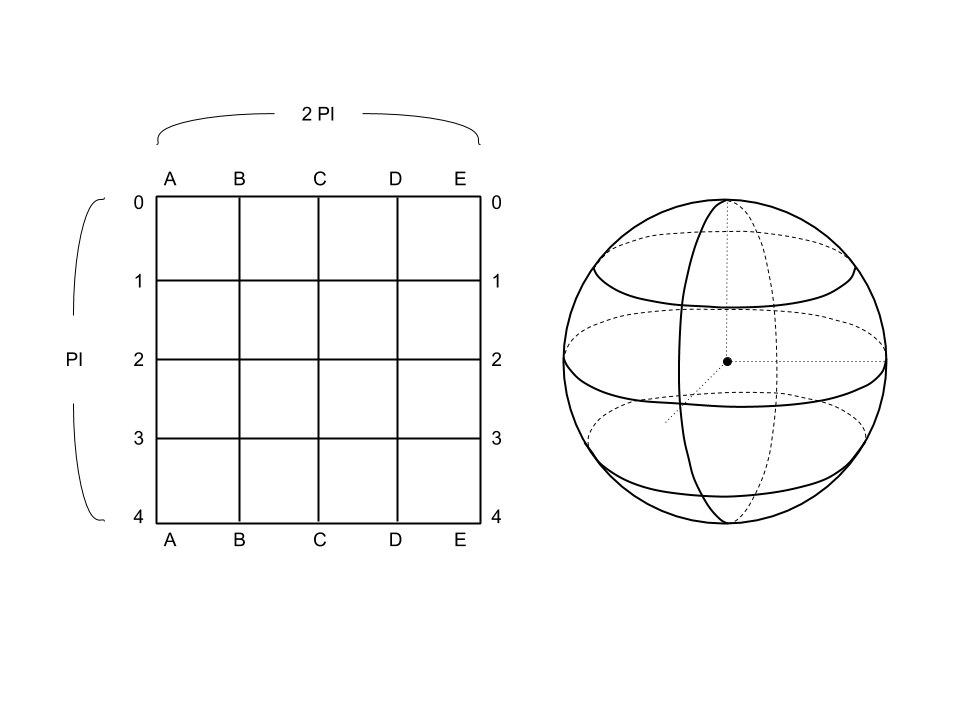
\includegraphics[width=\textwidth, keepaspectratio]{Figures/uv-sphere-mapping.png}
\decoRule
\end{figure}

The Diagram \ref{fig:uv-sphere-mapping} illustrates the mapping from 2D plane to 3D UV sphere's surface which has $5$ rings and $4$ segments. As we can seen, vertex $A0$, $A1$, $A2$, $A3$, $A4$ and $E0$, $E1$, $E2$, $E3$, $E4$ are duplicated; vertex $A0$, $B0$, $C0$, $D0$, $E0$ converge together in the pole, as well as $A4$, $B4$, $C4$, $D4$, $E4$. Also, in the UV sphere, each ring spans $2\,\pi$ radians, but each segment only spans $\pi$ radians.

The total vertex count for a UV sphere is:

\begin{equation}
\label{equ:uv-sphere-vertices}
\code{VerticesCount} = \code{RingsCount} \times \code{SegmentsCount}
\end{equation}

\begin{figure}[H]
\caption{UV sphere vertex}
\label{fig:uv-sphere-vertex}
\centering
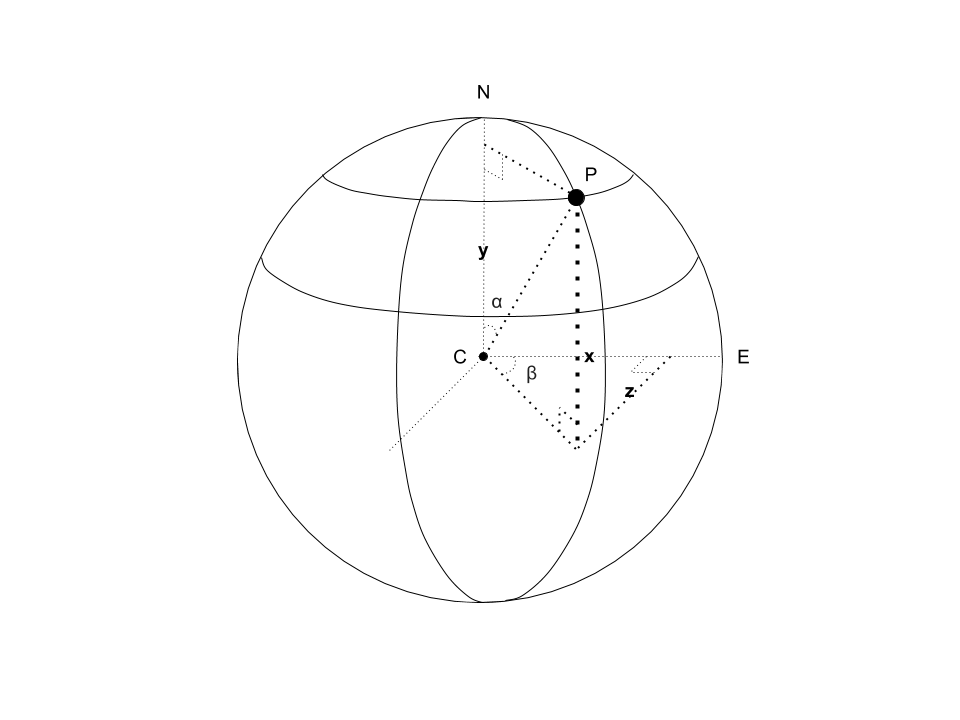
\includegraphics[width=\textwidth, keepaspectratio]{Figures/uv-sphere-vertex.png}
\decoRule
\end{figure}

If a vertex $P$ on the UV sphere belongs to ring $r$ and segment $s$:

\[
\begin{array}{lr}
v = r \times  \dfrac{1}{\code{RingsCount} - 1}\\\\
u = s \times  \dfrac{1}{\code{SegmentsCount} - 1}\\\\
\measuredangle \alpha = v \times \pi\\
\measuredangle \beta = u \times 2\,\pi\\
\end{array}
\]

$\therefore$ The vertex P (x,\;y,\;z) can be calculated:
\[
\begin{array}{lr}
x = (\sin(\alpha) \times radius) \times \cos(\beta)\\
y = \cos(\alpha) \times radius\\
z =  (\sin(\alpha) \times radius) \times \sin(\beta)\\
\end{array}
\]

The UV texturing (x,\;y) mapping for vertex $P$ is:

\[
\begin{array}{lr}
x = u\\
y = v\\
\end{array}
\]

It is vital to recognize the flip-side effect caused by the processing order of texturing. Diagram \ref{fig:uv-sphere-flip-side} shows a flip on the longitude direction. Which is not looking correct from outside of the Earth, but it is a precise mapping when the user is viewing from the inside.
 
\begin{figure}[H]
\caption{UV sphere flip-side effect}
\label{fig:uv-sphere-flip-side}
\centering
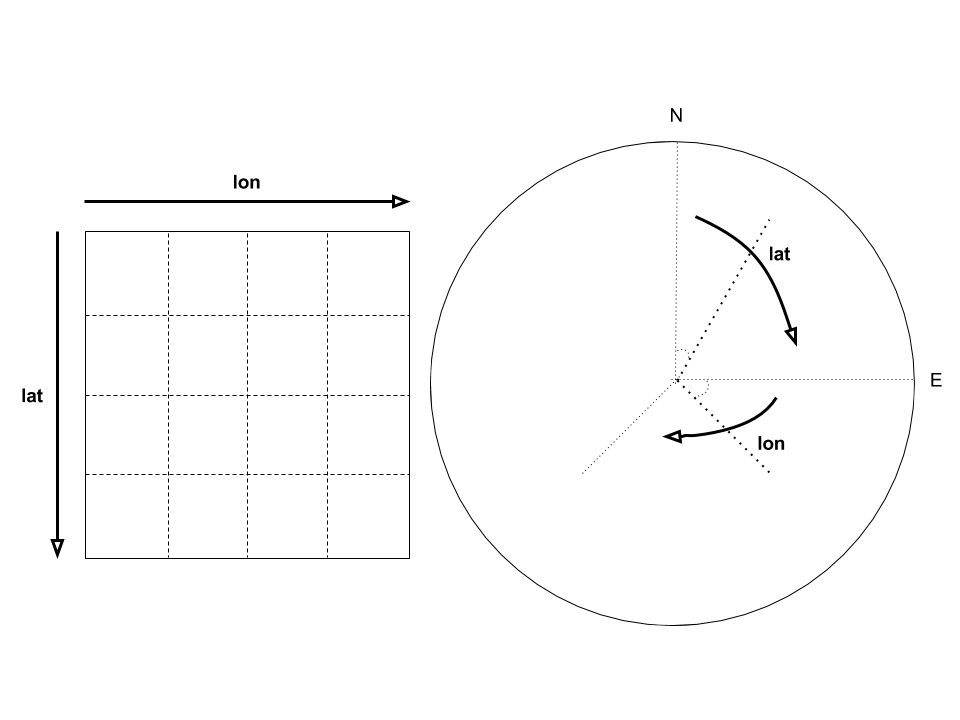
\includegraphics[width=\textwidth, keepaspectratio]{Figures/uv-sphere-flip-side.png}
\decoRule
\end{figure}

Given an ordering of each triangle's vertices, a triangle can appear to have a clockwise winding or counter-clockwise winding. Using OpenGL features Culling Face and Winding Order together to determine whether the triangle is visible from the front or the back side. In order to guarantee an inside visible only, \code{glFrontFace(GL\_CCW)} and \code{glCullFace(GL\_BACK)} can be adopted. The vertex indexes is ordered as Diagram \ref{fig:uv-sphere-ccw}.

\begin{figure}[H]
\caption{UV sphere CCW}
\label{fig:uv-sphere-ccw}
\centering
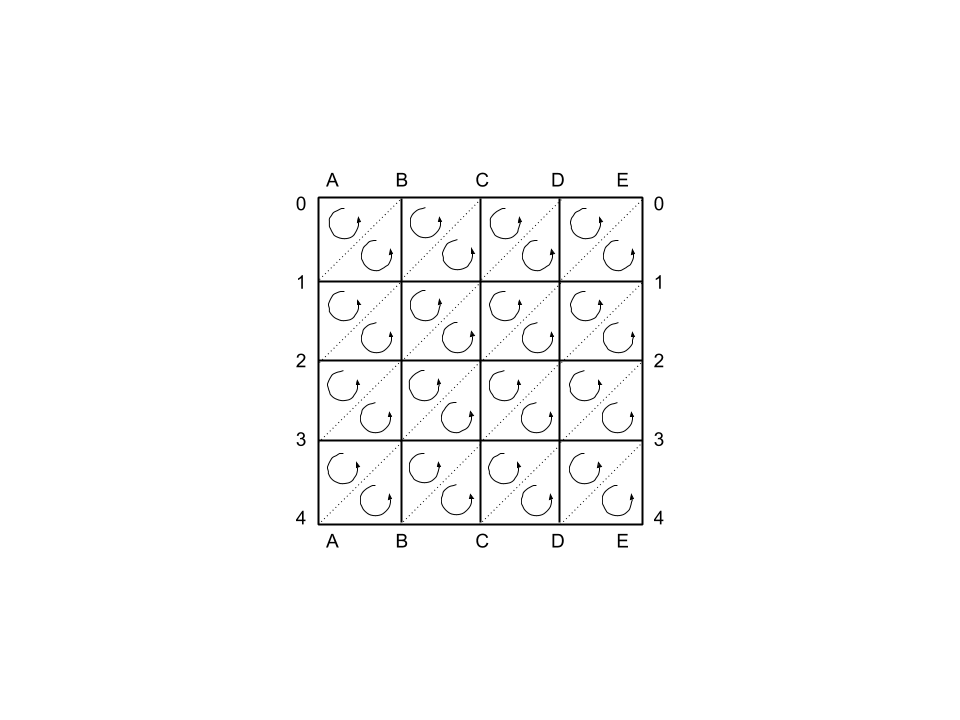
\includegraphics[width=\textwidth, keepaspectratio]{Figures/uv-sphere-ccw.png}
\decoRule
\end{figure}

%****************************************************************
\section{Placemark}

The vertex generation for \code{Placemark} is a recurring process of subdividing icosphere. Figure \ref{fig:icosahedron-rectangles} is an icosahedron, the corners of three orthogonal rectangles are the initial vertices for \code{Placemark}.

\begin{figure}[H]
\caption[Icosahedron rectangles]{Icosahedron rectangles \cite{wiki.icosahedron-rectangles.2006}}
\label{fig:icosahedron-rectangles}
\centering
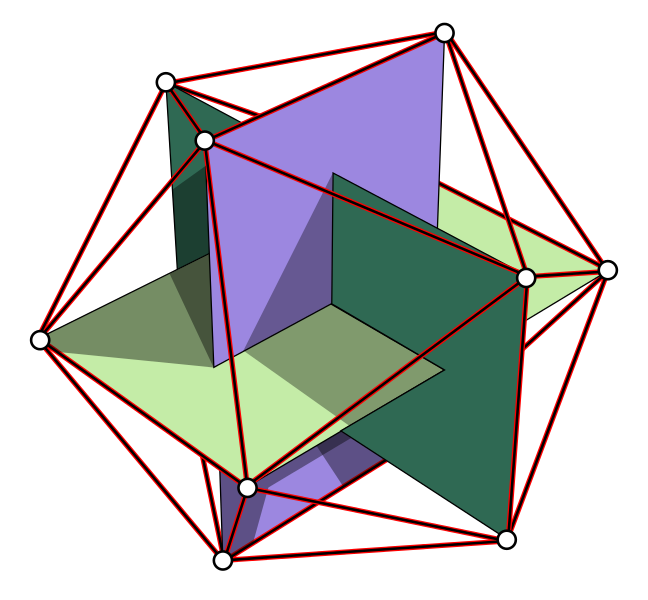
\includegraphics[width=0.7\textwidth, keepaspectratio]{Figures/icosahedron-rectangles.png}
\decoRule
\end{figure}

Rounding the icosphere by subdividing a face to an arbitrary level of resolution \ref{tab:icosphere-level}. Each face can be subdivided into four by connecting each edge's midpoint, then push the midpoints to the surface of the sphere \ref{fig:icosphere-refinement}.

\begin{figure}[H]
\caption{Icosphere refinement}
\label{fig:icosphere-refinement}
\centering
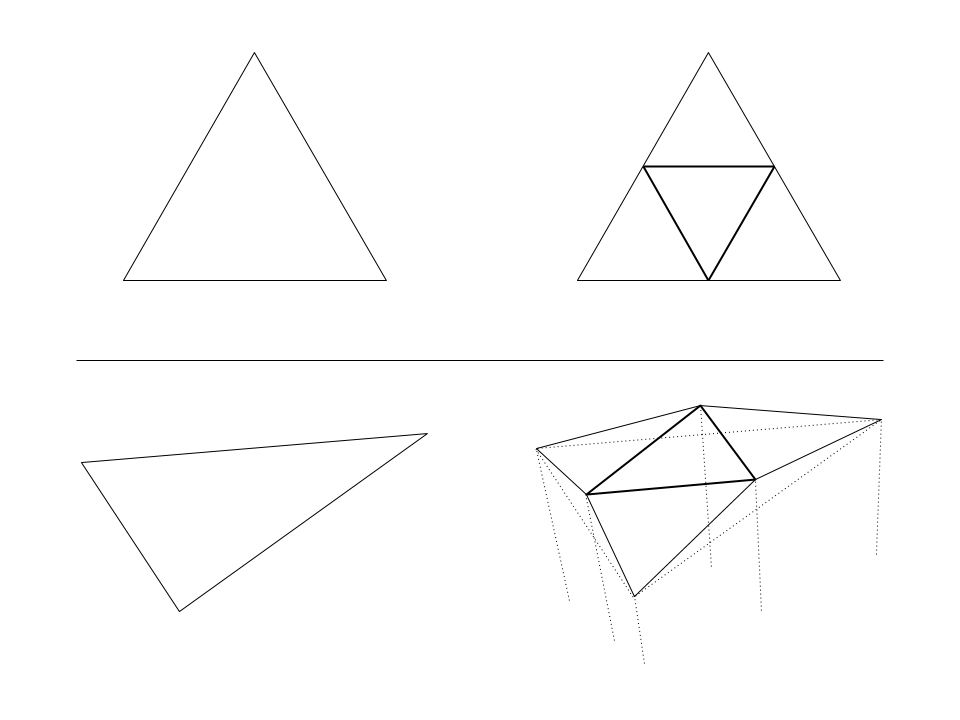
\includegraphics[width=\textwidth, keepaspectratio]{Figures/icosphere-refinement.png}
\decoRule
\end{figure}

First, get the midpoint of each edge.

\[
\begin{array}{lr}
\overrightarrow{d} = \dfrac{\overrightarrow{A} + \overrightarrow{B}}{2}\\\\
\overrightarrow{e} = \dfrac{\overrightarrow{A} + \overrightarrow{C}}{2}\\\\
\overrightarrow{f} = \dfrac{\overrightarrow{B} + \overrightarrow{C}}{2}\\
\end{array}
\]

Second, push midpoints to the surface of the unit sphere(1).

\[
\begin{array}{lr}
\overrightarrow{D} = \code{normalize}(\overrightarrow{d})\\
\overrightarrow{E} = \code{normalize}(\overrightarrow{e})\\
\overrightarrow{F} = \code{normalize}(\overrightarrow{f})\\
\end{array}
\]

Third, Also, adjustment of triangle's index array is required. Remove \code{$\triangle$ABC} in the vertex indexes list, add new \code{$\triangle$ADE}, \code{$\triangle$DBF}, \code{$\triangle$EFC}, and \code{$\triangle$DEF}.

\begin{figure}[H]
\caption{Icosphere vertex index}
\label{fig:icosphere-vertex-index}
\centering
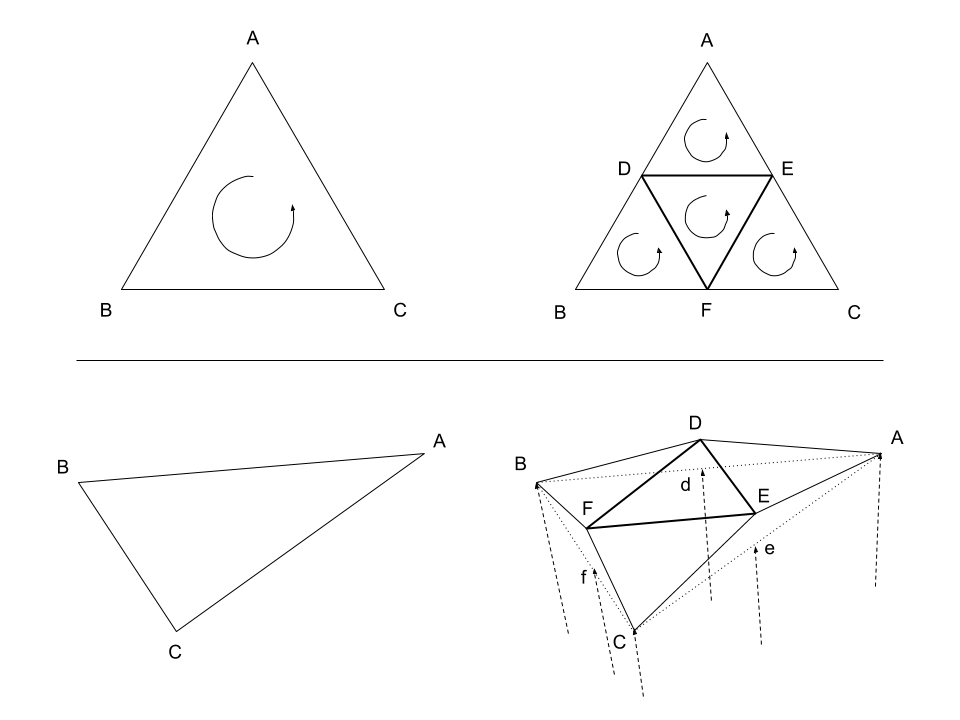
\includegraphics[width=\textwidth, keepaspectratio]{Figures/icosphere-vertex-index.png}
\decoRule
\end{figure}

Finally, draw the \code{Placemark} that looks the same size regardless of the distance in perspective view.

%****************************************************************
\subsection{Geographic Coordinate System}

The Earth geographic coordinate system is a coordinate system that enables everywhere on the Earth to be specified by a set of numbers or symbols \cite{wiki.geographic-coordinate-system.2016}. A common geodetic mapping coordinates are latitude, longitude, and altitude (LLA), which also is the raw location data decorated in KML file.

However, the LLA coordinates cannot be directly used from a program. Therefore, I introduce "earth-centered, earth-fixed" (ECEF) coordinate system for converting LLA coordinates to position coordinates. As we can see from Diagram \ref{fig:ecef}, the origin of the axis (0, 0, 0) is located at the center of the Earth, the z-axis and y-axis are pointing towards the north and east, and the x-axis intersects the Earth at $0$ latitude and $0$ longitude.

\begin{figure}[H]
\caption[ECEF]{Earth-centered, earth-fixed \cite{wiki.ecef.2016}}
\label{fig:ecef}
\centering
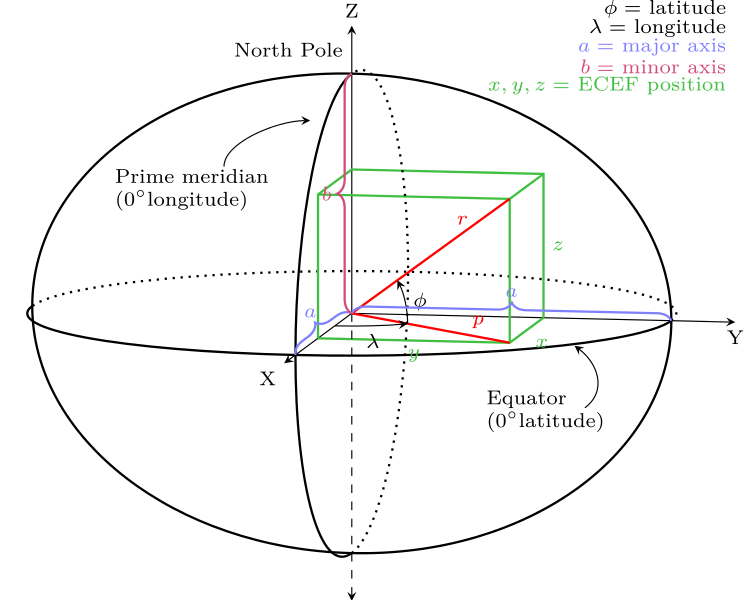
\includegraphics[width=\textwidth, keepaspectratio]{Figures/ecef.png}
\decoRule
\end{figure}

The ECEF coordinates are expressed in a reference system that is tended to be associated with geodetic mapping representations. In a system that practically requires high precision,  an accurate method to approximate the Earth’s shape is required. There have been researches on the elliptical earth since the 1980s. Nowadays, The new World Geodetic System was called WGS 84 which is currently being used by the Global Positioning System (GPS). It is geocentric and globally consistent within $\pm{1}$m. The WGS 84 has a series of parameters (table \ref{tab:wgs-84-parameters}) that define the shape of the ellipsoid (the Earth), they include a semi-major axis ($a$), a semi-minor axis ($b$) \ref{fig:ellipsoid-parameters}, its first eccentricity ($e_1$) and its second eccentricity ($e_2$).

\begin{figure}[H]
\caption{Ellipsoid parameters}
\label{fig:ellipsoid-parameters}
\centering
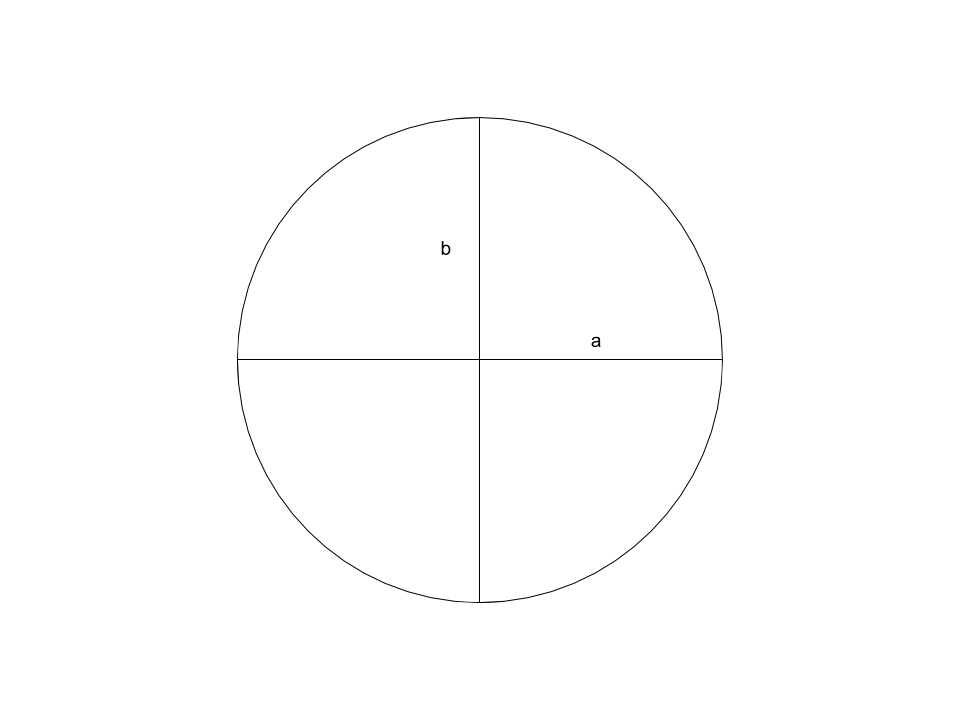
\includegraphics[width=\textwidth, keepaspectratio]{Figures/ellipsoid-parameters.png}
\decoRule
\end{figure}

\begin{table}[H]
\caption{WGS 84 parameters}
\label{tab:wgs-84-parameters}
\centering
	\begin{tabular}{l l l}
	\toprule
	\tabhead{Parameter} & \tabhead{Notation} & \tabhead{Value}\\
	\midrule
		Reciprocal of flattening & $\dfrac{1}{f}$ & 298.257\,223\,563\\
		Semi-major axis & $a$ & 6\,378\,137\,m\\
		Semi-minor axis & $b$ & $a\,(1 - f)$\\\\
		First eccentricity squared & $e_1^2$ & $1 - \dfrac{b^2}{a^2} = 2\,f - f^2$\\\\
		Second eccentricity squared & $e_2^2$ & $\dfrac{a^2}{b^2} - 1 = \dfrac{f\,(2 - f)}{(1 - f)^2}$\\
	\bottomrule
	\end{tabular}
\end{table}

In this application, where high accuracy is not required, simply using $a$ equals to $b$ (equals to the radius of the sphere). The conversion from LLA to ECEF as follow. 

\begin{figure}[H]
\caption{LLA to ECEF}
\label{fig:lla2ecef}
\centering
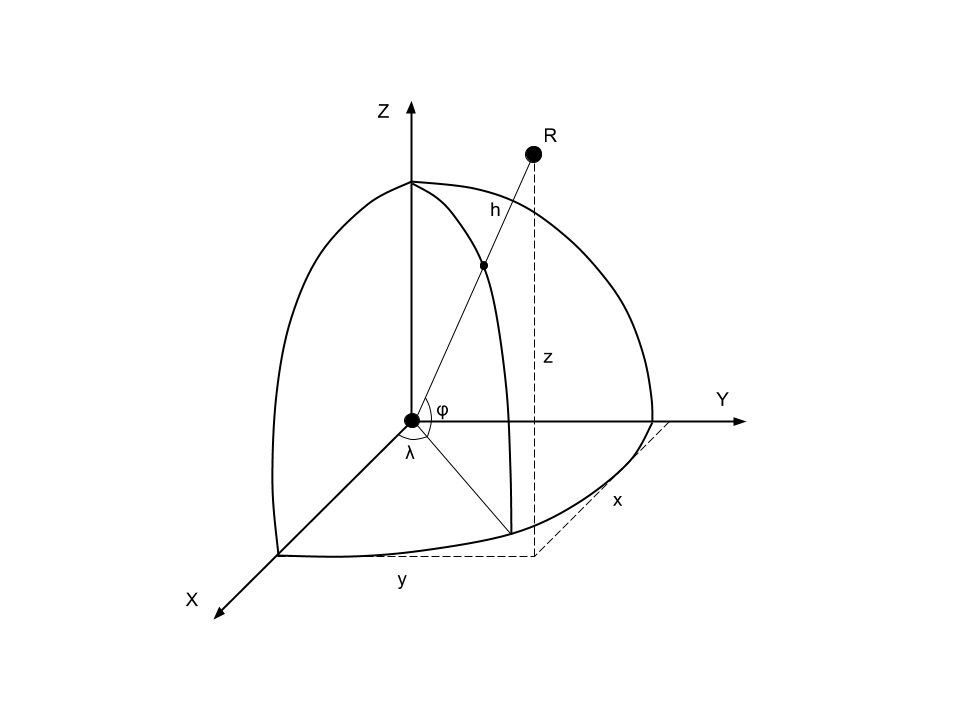
\includegraphics[width=\textwidth, keepaspectratio]{Figures/lla2ecef.png}
\decoRule
\end{figure}

\[
\begin{array}{lr}
\begin{aligned}
x &= (\mathbf{N} + \mathbf{h})\,\cos(\varphi)\,\cos(\lambda)\\
y &= (\mathbf{N} + \mathbf{h})\,\cos(\varphi)\,\sin(\lambda)\\
z &= (\dfrac{b^2}{a^2}\,\mathbf{N} + \mathbf{h})\,\sin(\varphi)\\
\end{aligned}
\end{array}
\]

Where;

\[
\begin{array}{lr}
\begin{aligned}
\varphi &= \code{Latitude}\\
\lambda &= \code{Longitude}\\
\mathbf{h} &= \code{Altitude}\\
\mathbf{N} &= \code{Radius of Curvature}\\
&= \dfrac{a}{\sqrt{1 - e^2\,\sin(\varphi)^2}}\\
\end{aligned}
\end{array}
\]

The final transformation from the ECEF to program graphic coordinates. This is relevant to how texture mapping and graphic system be implemented.

\[
\begin{array}{lr}
\begin{aligned}
\code{(x, y, z)}:\;&\text{y-east, z-north (up), x points to $0$ latitude and $0$ longitude}.\\
\Downarrow\;&\text{Reversal x, and switch z and y}.\\
\code{(-x, z, y)}:\;&\text{x-east, y-north (up), z points to $0$ latitude and $180$ longitude}.\\
\end{aligned}
\end{array}
\]

%****************************************************************
\subsection{Description}

The raw description data of a \code{Placemark} decorated in KML file is a series of characters that could include any URL. Therefore, an analysis of the description is required before transforming for display. In this application, it currently supports following information display.

\begin{description}
\setlength{\parskip}{0pt}
\item[$\bullet$ Plain text] Display the raw description data.
\item[$\bullet$ Image] Display the image from the URL.
\item[$\bullet$ Wikipedia] Display a extracted explanation on the topic.
\item[$\bullet$ HTML] Display \code{title} and \code{og:description} (one of the Open Graph metadata tags \cite{ogp.2014}) data (if it exists).
\end{description}

\begin{figure}[H]
\caption{Description analysis}
\label{fig:description-analysis}
\centering
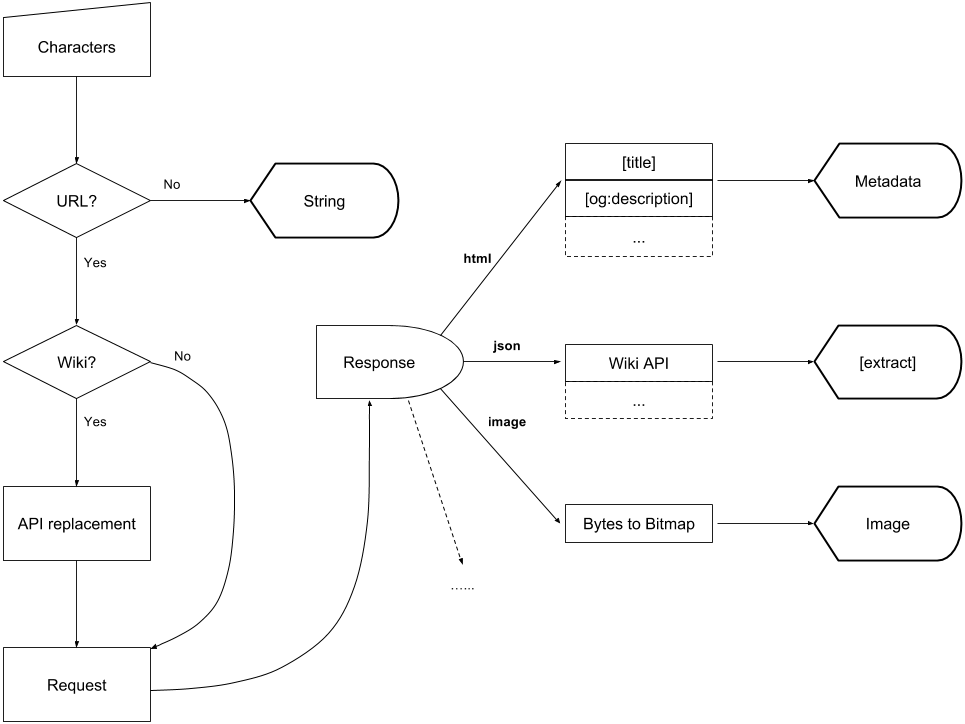
\includegraphics[width=\textwidth, keepaspectratio]{Figures/description-analysis.png}
\decoRule
\end{figure}

Treat the raw description data as plain text if it does not have a URL included. The\;\code{Content-Type} from the response of URL request, defines what kind of byte data is coming over, such as \code{image/jpeg}, \code{application/json}, or \code{text/html}. I am using Jsoup (a Java library for working with real-world HTML \cite{joup.2016}) for extracting target data from the HTML source. The most efficient way to get an extracted explanation or description on the topic from a Wikipedia page is to take use of the Opensearch API \cite{wiki.api.2016}. Therefore, a transformation from Wikipedia URL to Opensearch URL is required for an expected JSON response with \code{extract} tag included.

Given any valid Wikipedia page,

\[
\begin{array}{lr}
\begin{aligned}
\text{Replace}\;&\code{.wikipedia.org/wiki/}\\
&\Downarrow\\
\text{To}\;&\code{.wikipedia.org/w/api.php?}\textbf{APIs}\\
\end{aligned}
\end{array}
\]

Where \textbf{APIs} is:

\[
\begin{array}{lr}
\begin{aligned}
&\;\;\code{format=json}\\
&\code{\&action=query}\\
&\code{\&redirects=1}\\
&\code{\&prop=extracts}\\
&\code{\&exintro=}\\
&\code{\&explaintext=}\\
&\code{\&indexpageids=}\\
&\code{\&titles=}\\
\end{aligned}
\end{array}
\]

For instance,

\[
\begin{array}{lr}
\begin{aligned}
\code{https://en.wikipedia.org/}&\code{wiki/Virtual\_reality}\\
&\Downarrow\\
\code{https://en.wikipedia.org/}&\code{w/api.php?}\\
&\;\;\code{format=json\&action=query\&redirects=1}\\
&\code{\&prop=extracts\&exintro=\&explaintext=}\\
&\code{\&indexpageids=\&titles=Virtual\_reality}\\
\end{aligned}
\end{array}
\]

%****************************************************************
\subsection{Extra Model}
\label{section:obj-model}

A \code{Placemark} offers an ability to display a particular model that can be decorated as a URL in the \code{ExtendedData} (an element for adding custom data to a KML feature). In the sample data, there are some Wavefront OBJ models \cite{wiki.obj.2016} are created by the Blender (free software) and being used in this application.

A simple OBJ parser is implemented, it yet supports a full OBJ features \cite{paulbourke.obj}, such as syntax \code{mtllib} and \code{usemtl} are ignored. However, the main features that contain vertex related data for the model creation are supported, see Table \ref{tab:obj-syntax}.

\begin{table}[H]
\caption{OBJ syntax}
\label{tab:obj-syntax}
\centering
\begin{tabular}{l l l}
	\toprule
	\tabhead{Starting character / word} & \tabhead{Meaning}\\
	\midrule
	\code{v} & Geometric vertices\\
	\code{vt} & Texture coordinates\\
	\code{vn} & Vertex normals\\
	\code{f} & Face, composed of \code{v} / \code{vt} (optional) / \code{vn} (optional)\\
	\bottomrule
\end{tabular}
\end{table}

%****************************************************************
\section{Ray}
\label{section:ray}

A sight indicator is displayed in the center of sight for tracking the user's eyes. It is important to understand that the immersive virtual reality device works with glass lenses. Therefore the centering is not exactly the center of both view container. There are There are different implementation on both eye's viewports to convert a world-space vertex into inverse-lens distorted screen space. As a result, the user can see a slightly overlapping effect if the ray indicator is not be placed in a right distance. This phenomenon exists in reality as well. People can either get a better look at on a distant object or the fingers near to eyes.

%****************************************************************
\subsection{Ray Pointer}
\label{section:ray-pointer}

I place a ray pointer on the surface of the objects. It guarantees a clear display on both ray pointer and the target that user is staring at. It is drawn as \code{GL\_POINTS}, but rounding to a ring shape (see Figure \ref{fig:ray-point2ring}) in Fragment Shader \cite{wiki.fragment-shader.2016} - programmable Shader stage.

\begin{figure}[H]
\caption{Ray point to ring}
\label{fig:ray-point2ring}
\centering
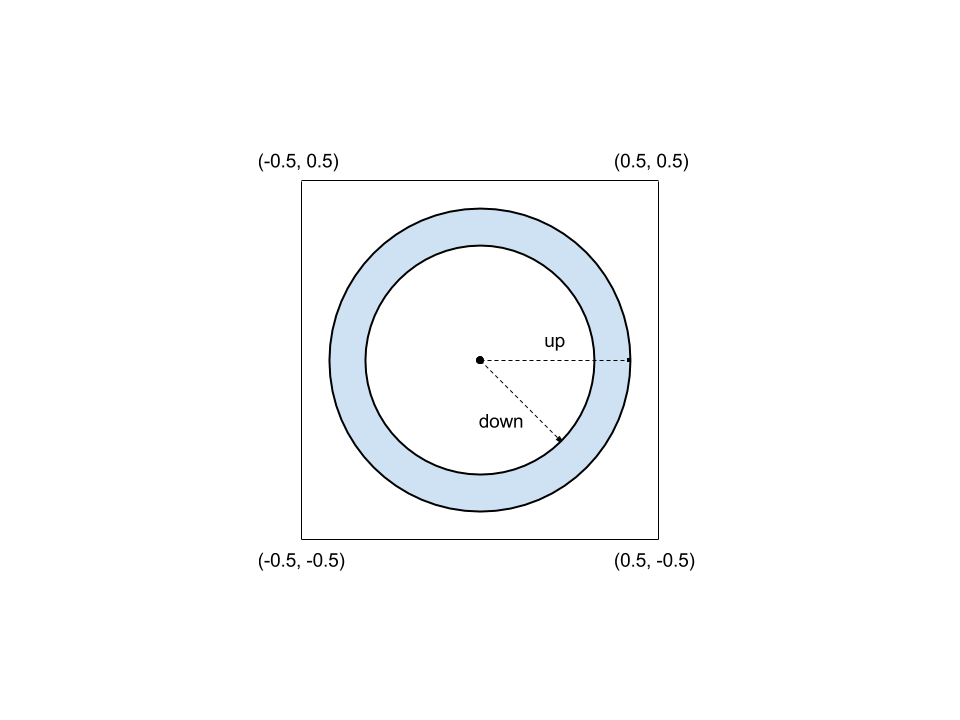
\includegraphics[width=\textwidth, keepaspectratio]{Figures/ray-point2ring.png}
\decoRule
\end{figure}

The \code{gl\_PointCoord} in the Fragment Shader has a range from $0$ to $1$ regardless of the point size. Therefore, center the point for circular calculation by shifting with $0.5$ offset on both x-axis and y-axis:

\[
\begin{array}{lr}
\begin{aligned}
&\code{// transform coord from range [0, 1] to [-0.5, 0.5]}\\
&\code{vec2 coord = gl\_PointCoord - vec2(0.5);}\\
\end{aligned}
\end{array}
\]

It is clear that a transformation from point to ring can be performed by ignoring invalid pixels in the point:

\[
\begin{array}{lr}
\begin{aligned}
&\code{float length = length(coord); // distance from the center}\\
&\code{bool belongsToPointer = pointerDown < length \&\& length < pointerUp;}\\
\end{aligned}
\end{array}
\]

%****************************************************************
\subsection{Ray Spinner}
\label{section:ray-spinner}

A ray spinner is an indicator gives a user feedback when the user is staring at a target. The ray spinner has a ring shape, but it is rendered as a dynamical arc by the given radian.

\begin{figure}[H]
\caption{Ray ring to spinner}
\label{fig:ray-ring2spinner}
\centering
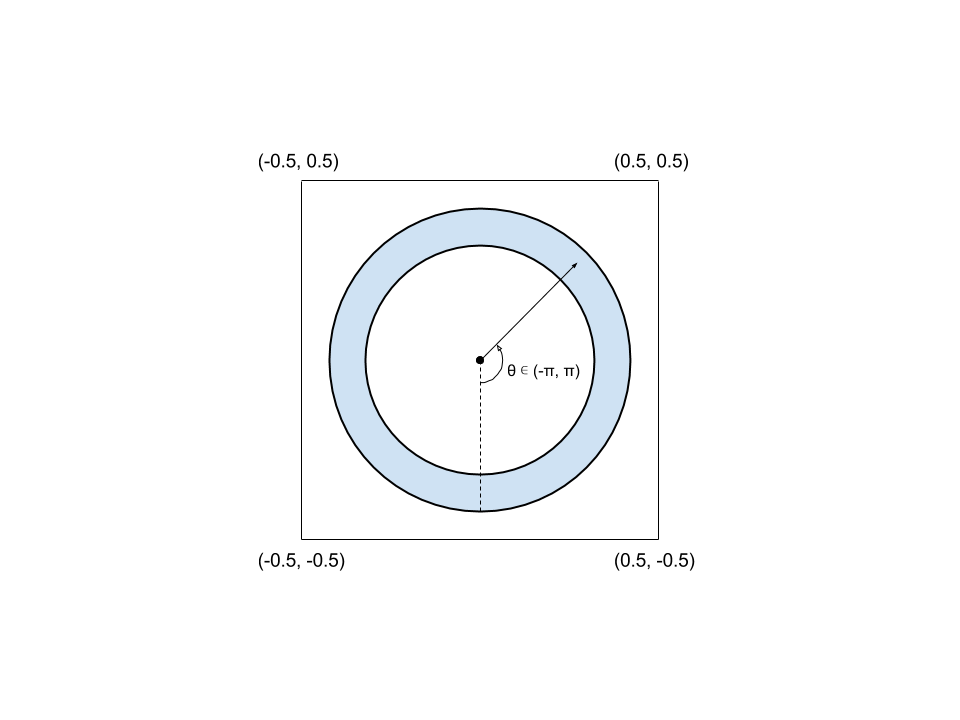
\includegraphics[width=\textwidth, keepaspectratio]{Figures/ray-ring2spinner.png}
\decoRule
\end{figure}

\[
\begin{array}{lr}
\begin{aligned}
&\code{bool belongsToSpinner = spinnerDown < length \&\& length < spinnerUp;}\\
&\code{float theta = atan (-coord.x, coord.y); //  (-PI, PI)}\\
&\code{belongsToSpinner = belongsToSpinner \&\& theta < u\_Spinner;}\\
\end{aligned}
\end{array}
\]

The \code{u\_Spinner} is a dynamical radian which came from CPU, and it has a range from $-\pi$ to $\pi$. The \code{genType atan(genType y, genType x)} returns the angle whose trigonometric arc tangent is $\dfrac{y}{x}$. The signs of \code{y} and \code{x} are used to determine the quadrant that the angle lies in. The value returned by \code{atan} is in the range from $-\pi$ to $\pi$.

%****************************************************************
\section{Information Display}

A flat plane 3D rectangular \code{Textfield} is implemented for displaying certain information, such as plain text and image. This information will be drawn as a texture and mapping to the \code{Textfield} vertex including the plain text. The calculation for the height of the total text with a certain pre-defined container width can be done by taking use of the Android native \code{android.text.StaticLayout}. 

The \code{Textfield} is been used for presenting details of \code{Placemark}, and the KML chooser menu. The menu which contains multiple \code{Textfield} that are laid out on the top of a 3D rectangular \code{Panel} with a small vertical dimension.

The vital part of the implementation for flat rectangular objects is to estimate and give them a right rotation (in front of eyes with zero relative rotation angle) based on the users' 3D head pose. Therefore, a head poses related quaternion matrix \cite{jvv.quaternions.2013} is needed to this end. I take the \code{head.quaternion} \code{(x, y, z, w)} provided by Google VR SDK from each frame, then convert the quaternion to a rotation matrix. First, reverse direction \code{(-x, -y, -z, w)} for facing to eye. Then, compute the rotation matrix by the given inhomogeneous expression \cite{wiki.quaternion-mat.2016}.

\begin{equation}
\label{equ:quaternion-matrix}
R = 
	\begin{bmatrix}
	1 - 2\,(q_z^2 + q_w^2) & 2\,(q_y\,q_z - q_x\,q_w) & 2\,(q_x\,q_z + q_y\,q_w)\\
	2\,(q_y\,q_z + q_x\,q_w) & 1 - 2\,(q_y^2 + q_w^2) & 2\,(q_z\,q_w - q_x\,q_y)\\
	2\,(q_y\,q_w - q_x\,q_z) & 2\,(q_x\,q_y + q_z\,q_w) & 1 - 2\,(q_y^2 + q_z^2)\\
	\end{bmatrix}
\end{equation}

%****************************************************************
\section{Camera Movement}

The ability to move around in virtual reality is important to satisfy user's need. Most Android-powered devices have built-in sensors that measure motion, orientation, and various environmental conditions \cite{google.sensors.2016}. The motion sensors measure acceleration forces and rotational forces along three axes. They include accelerometers, gravity sensors, gyroscopes, and rotational vector sensors. 

In general, the three physical axes (x, y, and z) data from Accelerometer sensor and Linear Acceleration sensor are useful to track and calculate device movement. Linear Acceleration is same as Accelerometer which measures the acceleration force in meter per second repeatedly, except the Linear Acceleration sensor is a synthetic sensor with gravity filtered out. 

\[
\begin{array}{lr}
\begin{aligned}
\code{LinearAcceleration} &= \code{Accelerometer} - \code{Gravity}\\
v &= \int a \cdot dt\\
x &= \int v \cdot dt\\
\end{aligned}
\end{array}
\]

However, there is a technical limitation. First of all, we take the accelerometer data and remove gravity that is called gravity compensation, whatever is left is linear movement. Then we have to integrate it once to get velocity, and integrated again to get the position, which is called double integral. If the first integral creates drift, the double integrals are nasty that they create horrible drift. In such noise, using acceleration data for navigation is not accurate, and it is hard to do any kind of linear movement \cite{google.sensor-fusion.2010}.

Therefore, I introduce Step Detector sensor and pedometer algorithm pedestrian navigation - user move forward on the current heading direction. First of all, during each frame life cycle, speed damping is calculated by a percentage stable and stop the camera in a certain of time regardless of current velocity. This is simply for avoiding that camera taking too long to stop. Secondly, each detected step causes a constant velocity pulse in the heading direction, see Diagram \ref{fig:camera-movement}.

\[
\begin{array}{lr}
p_1 = p_0 + v_0 \cdot dt\\
v_1 = v_0 + a \cdot dt\\
\end{array}
\]

\begin{figure}[H]
\caption{Camera movement}
\label{fig:camera-movement}
\centering
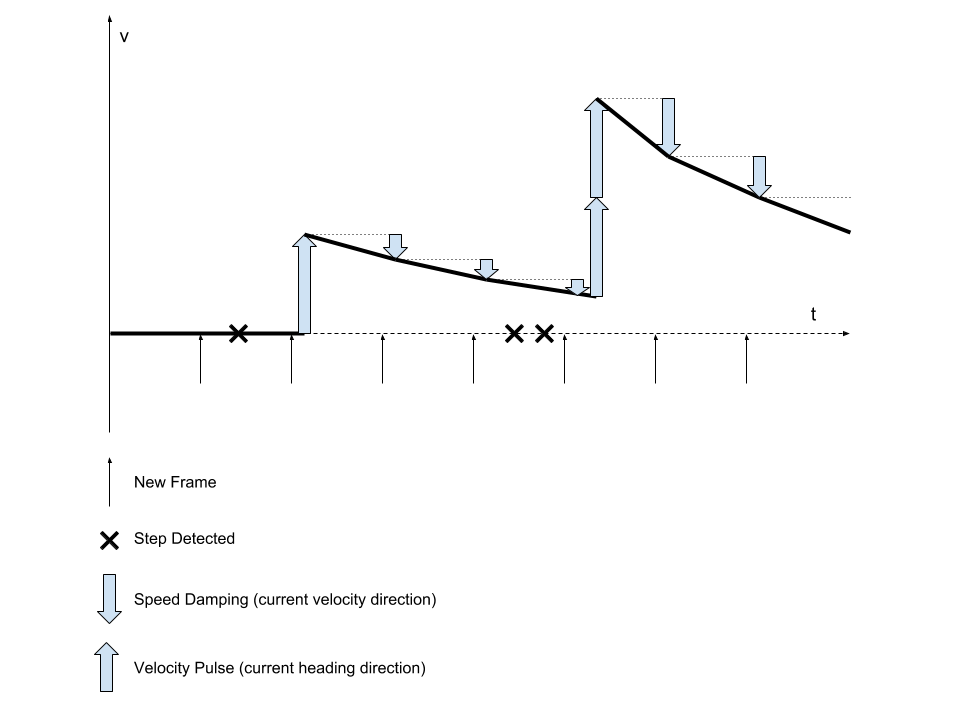
\includegraphics[width=\textwidth, keepaspectratio]{Figures/camera-movement.png}
\decoRule
\end{figure}

\[
\begin{array}{lr}
\begin{aligned}
\overrightarrow{V_0} &= \overrightarrow{V_0} \cdot \code{SpeedDamping}\\\\
\overrightarrow{P_1} &= \overrightarrow{P_0} + \overrightarrow{V_0} \cdot dt\\\\
\overrightarrow{V_1} &= \overrightarrow{V_0} + \overrightarrow{\code{HeadingDirection}} \cdot \code{Pulse} \cdot \code{DetectedStep}\\\\
\code{SpeedDamping} &\in [0,\enspace1]\\
\code{Pulse} &\in [0,\enspace \infty)\\
\end{aligned}
\end{array}
\]

%****************************************************************
\section{Ray Intersection}

In order to allow user interacts with virtual reality environment, the ability of intersection detection for ray-tracing is needed. In this way, it not only information can be easier present and understand, but also the user is able to interact (or select) objects in the 3D world.

A ray can be described in an equation with known starting position, $\overrightarrow{R_0}$ and its direction $\overrightarrow{R_d}$:

\begin{equation}
\label{equ:ray-t}
\overrightarrow{R(t)} = \overrightarrow{R_0} + \overrightarrow{R_d} \cdot t
\end{equation}

In this section, I separately reveal the intersection detection for basic elements. They are ray-sphere, ray-plane (3D rectangular), ray-box (2D and 3D).

%****************************************************************
\subsection{Ray-Sphere}
\label{section:ray-sphere}

\begin{figure}[H]
\caption{Ray-Sphere intersection}
\label{fig:ray-sphere}
\centering
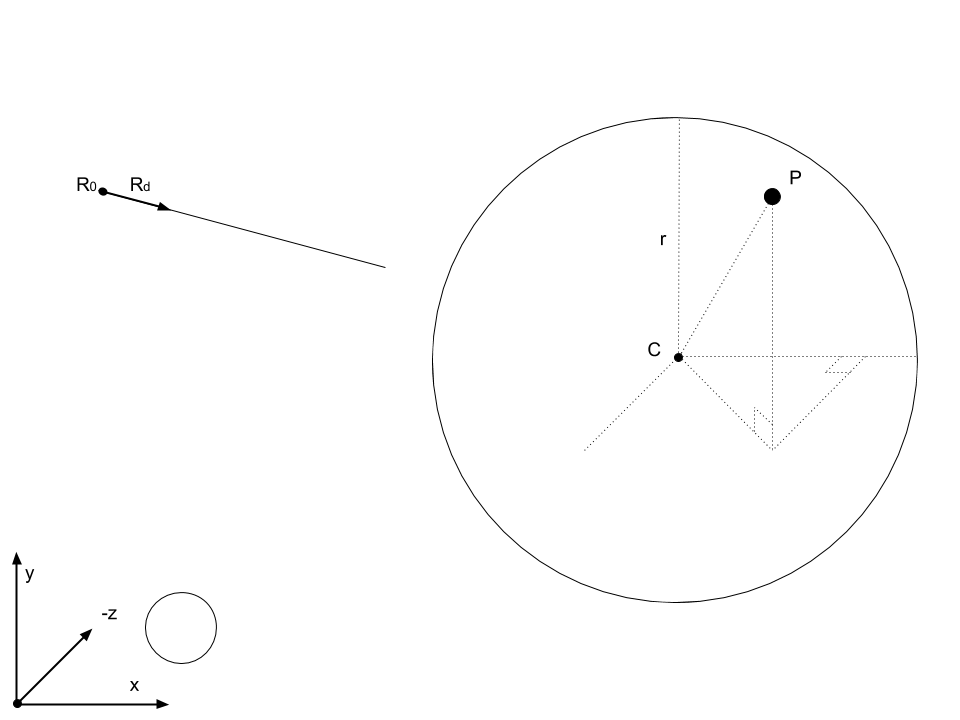
\includegraphics[width=\textwidth, keepaspectratio]{Figures/ray-sphere-intersection.png}
\decoRule
\end{figure}

A point $P$ on the surface of sphere can be described in an equation:

\begin{equation}
\label{equ:sphere-surface}
(x_p - x_c)^2 + (y_p - y_c)^2 + (z_p - z_c)^2 = r^2
\end{equation}

If the ray intersects with the sphere at any position $P$, it must match both equation \ref{equ:ray-t} and \ref{equ:sphere-surface}. Therefore the solution of $t$ from the cointegrate equation (as shown below) implies whether or not the ray will intersect with the sphere.

\[
\begin{aligned}
(x_{R_0} + x_{R_d} \cdot t - x_c)^2 + (y_{R_0} + y_{R_d} \cdot t - y_c)^2 &+ (z_{R_0} + z_{R_d} \cdot t - z_c)^2 &&= r^2\\
&\vdots\\
x_{R_d}^2\,t^2 + (2\,x_{R_d}\,(x_{R_0} - x_c))\,t &+ (x_{R_0}^2 - 2\,x_{R_0}\,x_c + x_c^2)\\
+\;y_{R_d}^2\,t^2 + (2\,y_{R_d}\,(y_{R_0} - y_c))\,t &+ (y_{R_0}^2 - 2\,y_{R_0}\,y_c + y_c^2)\\
+\;z_{R_d}^2\,t^2 + (2\,z_{R_d}\,(z_{R_0} - z_c))\,t &+ (z_{R_0}^2 - 2\,z_{R_0}\,z_c + z_c^2) &&= r^2\\
\end{aligned}
\]

It is essentially can be seen as a quadratic formula:

\begin{equation}
\label{equ:sphere-surface-quadratic-formula}
a\,t^2 + b\,t + c = 0
\end{equation}

Where the solution of $t$ are:

\begin{equation}
\label{equ:sphere-t-solution}
t =
\begin{cases}
\dfrac{-b \pm \sqrt{b^2 - 4\,a\,c}}{2\,a} & \text{if }\;b^2 - 4\,a\,c > 0\\\\
\dfrac{-b}{2\,a} & \text{if }\; b^2 - 4\,a\,c = 0\\\\
\varnothing & \text{if }\; b^2 - 4\,a\,c < 0\\
\end{cases}
\end{equation}

A further step to get rid of formula complexity by taking in geometric vector calculation.


$\because$\;\;\;\;Equation \ref{equ:sphere-surface} and equation \ref{equ:sphere-surface-quadratic-formula},

\[
\begin{array}{lr}
a = x_{R_d}^2 + y_{R_d}^2 + z_{R_d}^2\\
b = 2\,(x_{R_d}\,(x_{R_0} - x_c) + y_{R_d}\,(y_{R_0} - y_c) + z_{R_d}\,(z_{R_0} - z_c))\\
c = (x_{R_0} - x_c)^2 + (y_{R_0} - y_c)^2 + (z_{R_0} - z_c)^2 - r^2\\
\end{array}
\]

$\And$\;\;\;\;Geometric vector equation for $\overrightarrow{R_d}$ (ray's direction) and $\overrightarrow{V_c\_R_0}$ (vector from center of the sphere points to the ray's starting position):

\[
\begin{array}{lr}
\begin{aligned}
&\norm{\overrightarrow{R_d}} &&= \sqrt{x_{R_d}^2 + y_{R_d}^2 + z_{R_d}^2} = 1\\\\
&\overrightarrow{V_{c\_R_0}} &&= \overrightarrow{R_0} - \overrightarrow{C} = \overrightarrow{(x_{R_0} - x_c,\enspace y_{R_0} - y_c,\enspace z_{R_0} - z_c)}\\
\end{aligned}
\end{array}
\]

$\therefore$\;\;\;\;Value of $a$, $b$ and $c$ can be described as below:
\[
\begin{array}{lr}
a =1\\\\
b = 2 \cdot \overrightarrow{R_d} \cdot \overrightarrow{V_{c\_R_0}}\\\\
c = \overrightarrow{V_{c\_R_0}} \cdot \overrightarrow{V_{c\_R_0}} \cdot r^2\\
\end{array}
\]

$\And$\;\;\;\;Introducing $\alpha$ and $\beta$ to get rid of complexity for the equation \ref{equ:sphere-t-solution} of $t$:

\[
\begin{array}{lr}
\dfrac{-b \pm \sqrt{b^2 - 4\,a\,c}}{2\,a} = -\alpha \pm \sqrt{\beta}\\
\end{array}
\]

Where:

\[
\begin{array}{lr}
\begin{aligned}
\alpha &= \dfrac{1}{2}\,b\\
\beta &= \alpha^2 - c\\
\end{aligned}
\end{array}
\]

$\therefore$\;\;\;\;The solution formula for $t$ can also be optimized as below:

\[
t =
\begin{cases}
 -\alpha \pm \sqrt{\beta} & \text{if }\;\beta > 0\\
-\alpha & \text{if }\;\beta = 0\\
\varnothing & \text{if }\;\beta < 0\\
\end{cases}
\]

$\therefore$\;\;\;\;Given the known value of $\overrightarrow{R_0}$, $\overrightarrow{R_d}$ and $\overrightarrow{V_c}$, it is able to solve the $t$. The intersection position at any valid $t$ can be obtained as follow:

\[
\overrightarrow{P} = \overrightarrow{R_0} + \overrightarrow{R_d} \cdot t
\]

%****************************************************************
\subsection{Ray-Plane}

\begin{figure}[H]
\caption{Ray-Plane intersection}
\label{fig:ray-plane}
\centering
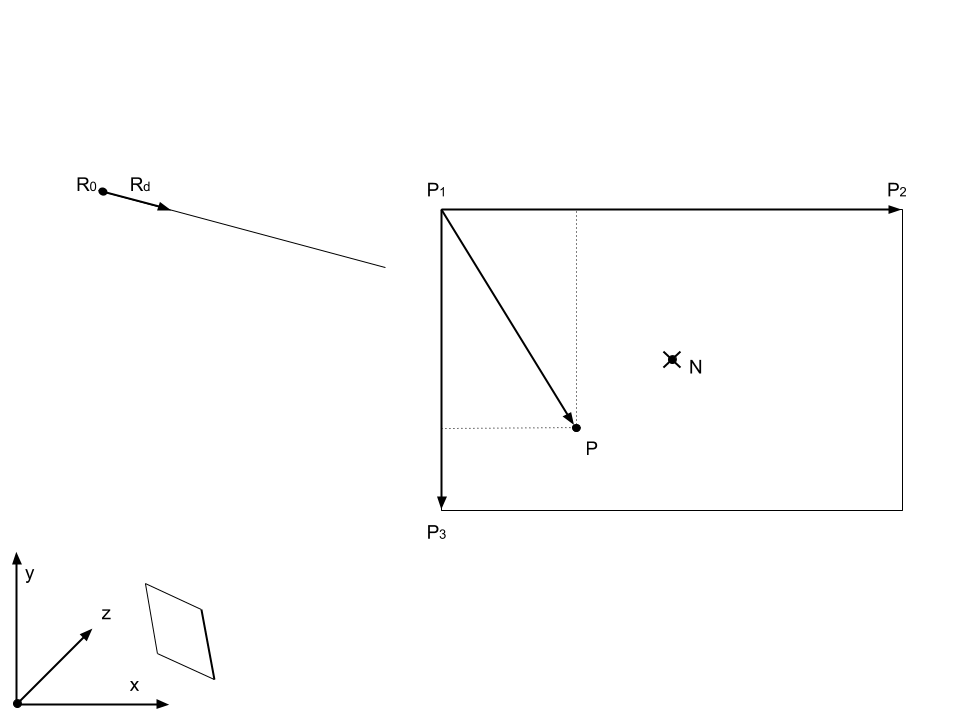
\includegraphics[width=\textwidth, keepaspectratio]{Figures/ray-plane-intersection.png}
\decoRule
\end{figure}

A point $P$ on the plane which means it perpendicular to the $\overrightarrow{N}$ of the plane. If the $P$ also belongs to the ray, then it can be described in a quadratic equation:

\begin{equation}
\label{equ:ray-plane-intersection}
\begin{array}{lr}
(\overrightarrow{P} - \overrightarrow{P_1}) \cdot \overrightarrow{N} = 0\\\\
\overrightarrow{P} = \overrightarrow{R_0} + \overrightarrow{R_d} \cdot t\\
\end{array}
\end{equation}

$\therefore$\;\;\;\;The solution for the $t$ is:

\[
t =
\begin{cases}
\dfrac{-\overrightarrow{N} \cdot (\overrightarrow{R_0} - \overrightarrow{P_1})}{\overrightarrow{N} \cdot \overrightarrow{R_d}} & \text{if }\;\overrightarrow{N} \cdot \overrightarrow{R_d} \nsim 0\;\;(\text{or} > \code{EPSILON})\\\\
\varnothing & \text{if }\;\overrightarrow{N} \cdot \overrightarrow{R_d} \sim 0\;\;(\text{or} < \code{EPSILON})\\
\end{cases}
\]

After all, taking a valid $t$ in equation \ref{equ:ray-plane-intersection} can only get the position $\overrightarrow{P}$ where the ray intersects with the plane. Therefore, we have to verify whether or not the $\overrightarrow{P}$ belongs to a specific rectangular with certain width and height. 

$\because$\;\;\;\;Given vector projection equation of $\overrightarrow{A}$ on $\overrightarrow{B}$:

\begin{equation}
\label{equ:vector-projection}
\begin{array}{lr}
A_{B} = \norm{A} \cdot \cos(\theta)\\\\
A_{B} = \dfrac{A \cdot B}{\norm{B}}\\
\end{array}
\end{equation}

$\therefore$\;\;\;\;The vector projection $\mu$ and $\nu$ of a valid $\overrightarrow{P}$ on both edges should greater than $0$ but smaller than the length of the edge.

\[
\begin{array}{lr}
\mu = \dfrac{(\overrightarrow{P} - \overrightarrow{P_1}) \cdot (\overrightarrow{P_2} - \overrightarrow{P_1})}{\enspace\norm{\overrightarrow{P_2} - \overrightarrow{P_1}}}\\\\
\nu = \dfrac{(\overrightarrow{P} - \overrightarrow{P_1}) \cdot (\overrightarrow{P_3} - \overrightarrow{P_1}))}{\norm{\overrightarrow{P_3} - \overrightarrow{P_1}}}\\\\
\mu \in [0,\enspace\norm{\overrightarrow{P_2} - \overrightarrow{P_1}}]\\
\nu \in [0,\enspace\norm{\overrightarrow{P_3} - \overrightarrow{P_1}}]\\
\end{array}
\]

Finally, transform them into a more optimized expression, and only if $\mu'$ and $\nu'$ satisfy the conditions below, the intersection position $\overrightarrow{P}$ is valid:

\[
\begin{array}{lr}
\mu' = (\overrightarrow{P} - \overrightarrow{P_1}) \cdot (\overrightarrow{P_2} - \overrightarrow{P_1})\\
\nu' = (\overrightarrow{P} - \overrightarrow{P_1}) \cdot (\overrightarrow{P_3} - \overrightarrow{P_1})\\
\mu' \in [0,\enspace (\overrightarrow{P_2} - \overrightarrow{P_1}) \cdot (\overrightarrow{P_2} - \overrightarrow{P_1})]\\
\nu' \in [0,\enspace (\overrightarrow{P_3} - \overrightarrow{P_1}) \cdot (\overrightarrow{P_3} - \overrightarrow{P_1})]\\
\end{array}
\]

%****************************************************************
\subsection{Ray-Box}
\label{section:ray-box}

See section \ref{section:space-partition}, space partition is implemented in the 3D world that separates the space to invisible boxes that each box may or may not contain other objects. Ray-box intersection implementation for avoids unnecessary ray-object intersection tests. In this section, explanation divided into two parts, ray-box in 2D and which have inspired to ray-box 3D implementation. In the current implementation, I assume the boxes are located aligned with the axis, which is exactly how space partition works. This limitation can be solved with a certain rotation transformation in advance.

%****************************************************************
\subsubsection{Ray-Box 2D}

\begin{figure}[H]
\caption{Ray-Box 2D intersection}
\label{fig:ray-box-2d}
\centering
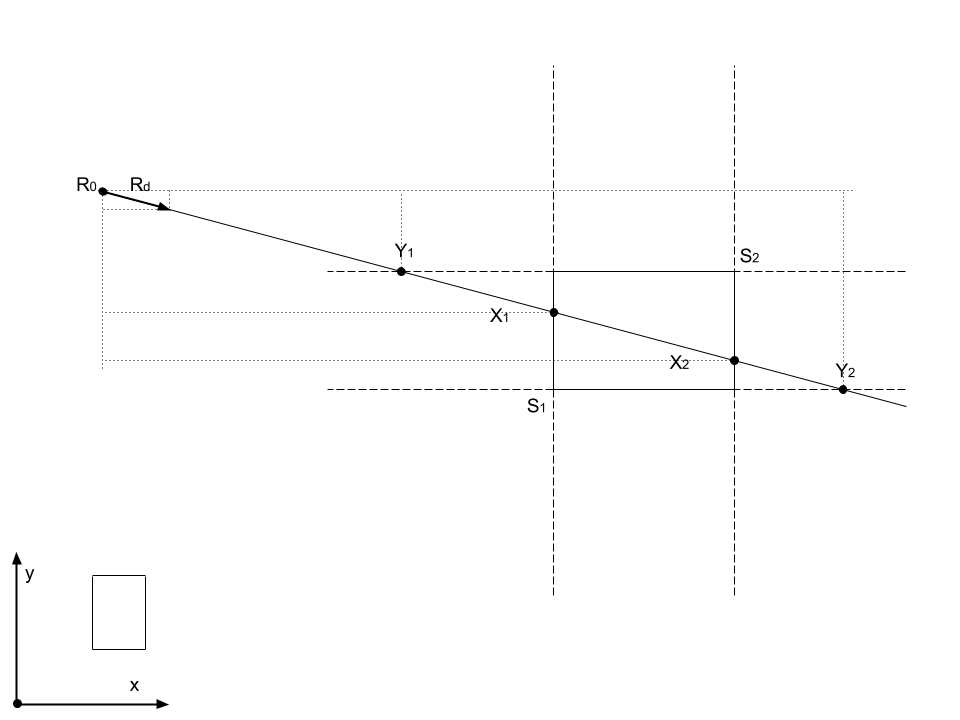
\includegraphics[width=\textwidth, keepaspectratio]{Figures/ray-box-2d-intersection.png}
\decoRule
\end{figure}

Given known $R_0$ (ray's starting position),\enspace$R_d$ (ray's direction),\enspace$P_1$ (left-bottom corner),\enspace$P_2$ (right-top corner), we can get the value of $X_1$,\enspace$X_2$,\enspace$Y_1$ and $Y_2$. When ray intersecting with the 2D box, they have such meaning:

\begin{description}
	\setlength{\parskip}{0pt}
	\item[$\bullet$ Vertical Area] Vertical route area between the left edge and right edge (include the area beyond the box)
	\item[$\bullet$ Horizontal Area] Horizontal route area between the top edge and bottom edge (include the area beyond the box)
	\item[$\bullet$ $\mathbf{X}_1$] The distance from $R_0$ to the "in" point of Vertical Area in the x-axis direction.   
	\item[$\bullet$ $\mathbf{X}_2$] The distance from $R_0$ to the "out" point of Vertical Area in the x-axis direction. 
	\item[$\bullet$ $\mathbf{Y}_1$] The distance from $R_0$ to the "in" point of Horizontal Area in the y-axis direction.
	\item[$\bullet$ $\mathbf{Y}_2$] The distance from $R_0$ to the "out" point of Horizontal Area in the y-axis direction. 
\end{description}

$\therefore$

\begin{multicols}{2}
\noindent
	\[
	X_1 =
	\begin{cases}
	x_{P_1} - x_{R_0} & \text{if }\;x_{R_d} > 0\\
	x_{P_2} - x_{R_0} & \text{if }\;x_{R_d} < 0\\
	\end{cases}
	\]
\columnbreak
	\[
	X_2 =
	\begin{cases}
	x_{P_2} - x_{R_0} & \text{if }\;x_{R_d} > 0\\
	x_{P_1} - x_{R_0} & \text{if }\;x_{R_d} < 0\\
	\end{cases}
	\]
\end{multicols}

\begin{multicols}{2}
\noindent
	\[
	Y_1 =
	\begin{cases}
	y_{P_1} - y_{R_0} & \text{if }\;y_{R_d} > 0\\
	y_{P_2} - y_{R_0} & \text{if }\;y_{R_d} < 0\\
	\end{cases}
	\]
\columnbreak
	\[
	Y_2 =
	\begin{cases}
	y_{P_2} - y_{R_0} & \text{if }\;y_{R_d} > 0\\
	y_{P_1} - y_{R_0} & \text{if }\;y_{R_d} < 0\\
	\end{cases}
	\]
\end{multicols}

$\And$\;\;\;\;The relative distance in x-axis and y-axis direction:

\begin{multicols}{2}
\noindent
	\[
	\begin{array}{lr}
	t_{X_1} = \dfrac{X_1}{x_{R_d}}\\\\
	t_{X_2} = \dfrac{X_2}{x_{R_d}}\\
	\end{array}
	\]
\columnbreak
	\[
	\begin{array}{lr}
	t_{Y_1} = \dfrac{Y_1}{y_{R_d}}\\\\
	t_{Y_2} = \dfrac{Y_2}{y_{R_d}}\\
	\end{array}
	\]
\end{multicols}

$\therefore$\;\;\;\;A valid intersection exist only if following equation satisfied:

\[
\begin{array}{lr}
\begin{aligned}
t_{X_1} &< t_{X_2}\\
t_{Y_1} &< t_{Y_2}\\
\end{aligned}
\end{array}
\]

Which is:

\[
\code{max}\;(t_{X_1},\enspace t_{Y_1}) < \code{min}\;(t_{X_2},\enspace t_{Y_2})
\]

%****************************************************************
\subsubsection{Ray-Box 3D}

\begin{figure}[H]
\caption{Ray-Box 3D intersection}
\label{fig:ray-box-3d}
\centering
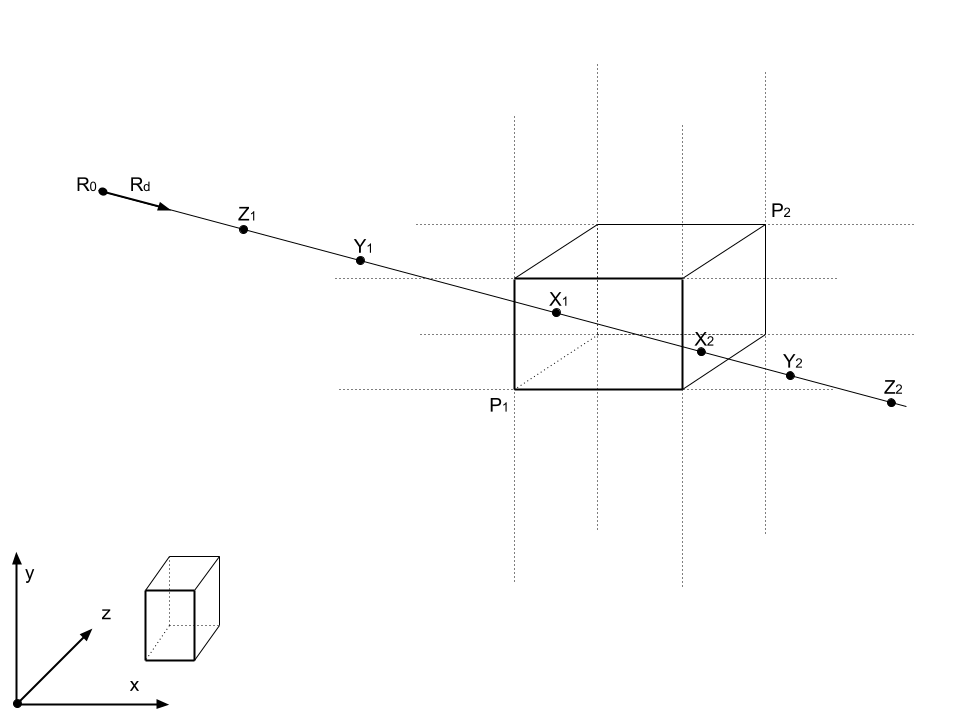
\includegraphics[width=\textwidth, keepaspectratio]{Figures/ray-box-3d-intersection.png}
\decoRule
\end{figure}

Given known $R_0$ (ray's starting position),\enspace$R_d$ (ray's direction),\enspace$P_1$ (left-bottom-front corner),\enspace$P_2$ (right-top-back corner), we can get the value of $X_1$,\enspace$X_2$,\enspace$Y_1$, $Y_2$, $Z_1$ and $Z_2$. When ray intersecting with the 3D box, they have such meaning:

\begin{description}
	\setlength{\parskip}{0pt}
	\item[$\bullet$ Vertical Area] Vertical route area within the scope of left-face, right-face, back-face and front face (include the area beyond the box)
	\item[$\bullet$ Horizontal Area] Horizontal route area within the scope of top-face, bottom-face, back-face and front face (include the area beyond the box)
	\item[$\bullet$ Z-depth Area] Z-depth route area within the scope of top-face, bottom-face, left-face and right face (include the area beyond the box)
	\item[$\bullet$ $\mathbf{X}_1$] The distance from $R_0$ to the "in" point of Vertical Area in the x-axis direction.   
	\item[$\bullet$ $\mathbf{X}_2$] The distance from $R_0$ to the "out" point of Vertical Area in the x-axis direction. 
	\item[$\bullet$ $\mathbf{Y}_1$] The distance from $R_0$ to the "in" point of Horizontal Area in the y-axis direction.
	\item[$\bullet$ $\mathbf{Y}_2$] The distance from $R_0$ to the "out" point of Horizontal Area in the y-axis direction. 
	\item[$\bullet$ $\mathbf{Z}_1$] The distance from $R_0$ to the "in" point of Z-depth Area in the z-axis direction.
	\item[$\bullet$ $\mathbf{Z}_2$] The distance from $R_0$ to the "out" point of Z-depth Area in the z-axis direction. 
\end{description}

$\therefore$

\begin{multicols}{2}
\noindent
	\[
	X_1 =
	\begin{cases}
	x_{P_1} - x_{R_0} & \text{if }\;x_{R_d} > 0\\
	x_{P_2} - x_{R_0} & \text{if }\;x_{R_d} < 0\\
	\end{cases}
	\]
\columnbreak
	\[
	X_2 =
	\begin{cases}
	x_{P_2} - x_{R_0} & \text{if }\;x_{R_d} > 0\\
	x_{P_1} - x_{R_0} & \text{if }\;x_{R_d} < 0\\
	\end{cases}
	\]
\end{multicols}

\begin{multicols}{2}
\noindent
	\[
	Y_1 =
	\begin{cases}
	y_{P_1} - y_{R_0} & \text{if }\;y_{R_d} > 0\\
	y_{P_2} - y_{R_0} & \text{if }\;y_{R_d} < 0\\
	\end{cases}
	\]
\columnbreak
	\[
	Y_2 =
	\begin{cases}
	y_{P_2} - y_{R_0} & \text{if }\;y_{R_d} > 0\\
	y_{P_1} - y_{R_0} & \text{if }\;y_{R_d} < 0\\
	\end{cases}
	\]
\end{multicols}

\begin{multicols}{2}
\noindent
	\[
	Z_1 =
	\begin{cases}
	z_{P_1} - z_{R_0} & \text{if }\;z_{R_d} > 0\\
	z_{P_2} - z_{R_0} & \text{if }\;z_{R_d} < 0\\
	\end{cases}
	\]
\columnbreak
	\[
	Z_2 =
	\begin{cases}
	z_{P_2} - z_{R_0} & \text{if }\;z_{R_d} > 0\\
	z_{P_1} - z_{R_0} & \text{if }\;z_{R_d} < 0\\
	\end{cases}
	\]
\end{multicols}

$\And$\;\;\;\;The relative distance in different axis direction:

\begin{multicols}{3}
\noindent
	\[
	\begin{array}{lr}
	t_{X_1} = \dfrac{X_1}{x_{R_d}}\\\\
	t_{X_2} = \dfrac{X_2}{x_{R_d}}\\
	\end{array}
	\]
\columnbreak
	\[
	\begin{array}{lr}
	t_{Y_1} = \dfrac{Y_1}{y_{R_d}}\\\\
	t_{Y_2} = \dfrac{Y_2}{y_{R_d}}\\
	\end{array}
	\]
\columnbreak
	\[
	\begin{array}{lr}
	t_{Z_1} = \dfrac{Z_1}{z_{R_d}}\\\\
	t_{Z_2} = \dfrac{Z_2}{z_{R_d}}\\
	\end{array}
	\]
\end{multicols}

$\therefore$\;\;\;\;A valid intersection exist only if following equation satisfied:

\[
\begin{array}{lr}
\begin{aligned}
t_{X_1} &< t_{X_2}\\
t_{Y_1} &< t_{Y_2}\\
t_{Z_1} &< t_{Z_2}\\
\end{aligned}
\end{array}
\]

$\therefore$ Which is:

\begin{equation}
\label{equ:ray-box-3d-intersection}
\code{max}\;(t_{X_1},\enspace t_{Y_1},\enspace t_{Z_1}) < \code{min}\;(t_{X_2},\enspace t_{Y_2},\enspace t_{Z_2})
\end{equation}

%****************************************************************
